%
% This document is licensed under the
%
%   Creative Commons Attribution-Noncommercial-Share Alike
%
% license. Please see LICENSE file for details.
%

%
% Complete documentation on the extended LaTeX markup used for Insight
% documentation is available in ``Documenting Insight'', which is part
% of the standard documentation for Insight.  It may be found online
% at:
%
%     http://www.itk.org/

\documentclass{InsightArticle}

\usepackage[dvipdfm]{graphicx}
\usepackage{url}

%%%%%%%%%%%%%%%%%%%%%%%%%%%%%%%%%%%%%%%%%%%%%%%%%%%%%%%%%%%%%%%%%%
%
%  hyperref should be the last package to be loaded.
%
%%%%%%%%%%%%%%%%%%%%%%%%%%%%%%%%%%%%%%%%%%%%%%%%%%%%%%%%%%%%%%%%%%
\usepackage[dvipdfm,
bookmarks,
bookmarksopen,
backref,
colorlinks,linkcolor={blue},citecolor={blue},urlcolor={blue},
]{hyperref}


%  This is a template for Papers to the Insight Journal. 
%  It is comparable to a technical report format.

% The title should be descriptive enough for people to be able to find
% the relevant document. 
\title{User Guide to \\[4mm] The Computational Morphometry
  Toolkit\footnote{This document is licensed under
    the Creative Commons Attribution-Noncommercial-Share Alike (CC-NC-SA) license}}

% Increment the release number whenever significant changes are made.
% The author and/or editor can define 'significant' however they like.
\release{1.00}

% At minimum, give your name and an email address.  You can include a
% snail-mail address if you like.
\author{Torsten Rohlfing}
\authoraddress{Neuroscience Program, SRI International, Menlo Park, CA\footnote{Continued development and maintenance of CMTK is funded by
    the NIBIB under Grant No. R01~EB008381.}}

\begin{document}

\maketitle

\ifhtml
\chapter*{Front Matter\label{front}}
\fi


% The abstract should be a paragraph or two long, and describe the
% scope of the document.
\begin{abstract}
\noindent
This paper is intended as a very brief introduction of the main tools in the
Computational Morphometry Toolkit (CMTK). The target audience are CMTK users,
who might use this codument as a reference to the most common processing
tasks, and prospective users, who may find this information useful to
determine whether CMTK provides functionality that they can use.
\end{abstract}

\clearpage
\tableofcontents
\clearpage


\section{Introduction}

The Computational Morphometry Toolkit, or short CMTK, is a set of software
tools that perform various types of processing and analysis on
three-dimensional (3D) image data. CMTK is available both in source code
(licensed under the GNU GPL3) and as pre-compiled binaries from
\url{http://www.nitrc.org/projects/cmtk/}.

CMTK is primarily a collection of command line tools, which make the toolkit
ideally suited for unattended batch processing of large amounts of data. In
addition, CMTK's backend libraries, which are shared by all command line
tools, can be used as a relatively lightweight, yet powerful, platform for
implementation of new image processing algorithms.

\subsection{Coordinate Conventions}

For medical image data, CMTK uses an anatmoy-based coordinate system, which we
refer to as ``RAS'' coordinates. This means that the $x$ direction of the
coordinate space increases towards the anatomical ``Right,'' the $y$ direction
increases towards the anatomical ``Anterior,'' and the $z$ direction increases
towards the anatomical ``Superior.'' The coordinate space origin, $(0,0,0)$,
thus coincides with the ``Left-Posterior-Inferior'' corner of the image
volume. 

All images that are read into one of CMTK's tools are first reoriented to fit
this coordinate system. This means that the storage order of image pixels in
memory is such that the fastest-varying of the three pixel indexes corresponds
to the ``Left''--''Right'' anatomical direction, the second fastest to the
``Posterior''--''Anterior'' direction, and the slowest varying to the
``Inferior''--''Superior'' direction. Consequently, the first pixel in memory
is the one that is the Left-Posterior-Inferior-most pixel anatomically.

For image file formats that define subject orientation based on direction
vectors within an anatomy-based coordinate space, which is the majority of
modern formats, CMTK determines the nearest anatomical orientation of the
image within $\pm 45$ degrees around each rotation axis.

To confirm that images are read correctly, and to diagnose problems, CMTK
comes with a very simple triplanar image viewer (see screenshot in
Fig.~\ref{fig:triplanar}), adequately named ``\verb|triplanar|.'' The
coordinates shown in this viewer for any image are exactly the coordinates
that all CMTK tools use. Note that for the triplanar viewer to be available,
CMTK must be built with support for the Qt
toolkit\footnote{\url{http://qt.nokia.com}} (version 4.3.0 or higher), and the
``\verb|BUILD_GUI|'' build option must be enabled.

\begin{figure}[tbp]
\centerline{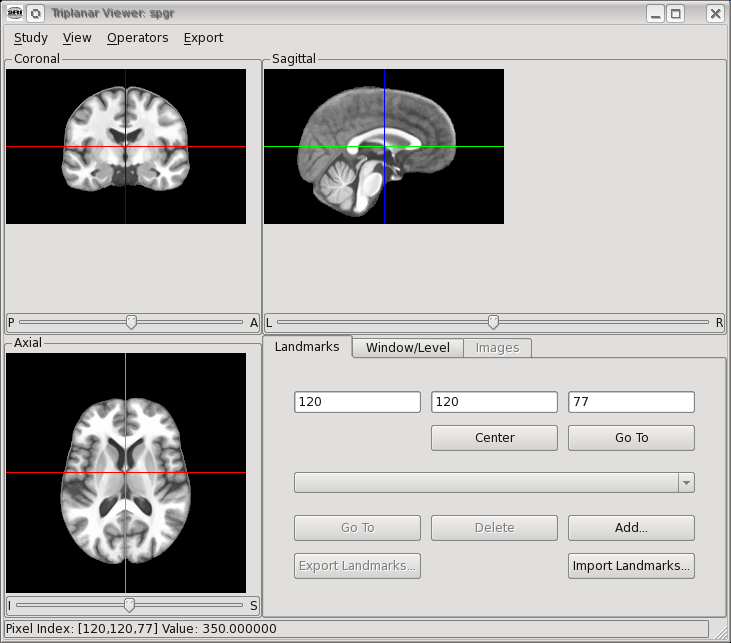
\includegraphics[width=.5\linewidth]{img/triplanar}}
\caption{Screenshot of CMTK's triplanar image viewer.}
\label{fig:triplanar}
\end{figure}

\subsection{Registration Terminology}

Since one of the primary strenghts of CMTK is its selection of powerful and
well-tested registration tools, we shall first clarify some important
registration terminology. In pairwise registration, throughout this guide as
well as in all tools and source code, we shall refer to one image as the
reference and the other as the floating image. Others may refer to these as
the fixed and the moving image, respectively. By definition, all coordinate
transformations computed by CMTK are functions that map {\em from\/} the space
of the reference (fixed) image {\em to\/} the space of the floating (moving)
image. As a result, when reformatting one image to match the other, it is the
floating image by default that will be transformed to match the reference
image.

Note that when we speak about transforming coordinates of features, such as
landmarks or the nodes in a mesh, then the coordinates of the reference image
will be transformed to match the floating image.

\subsection{Supported Image File Formats}

CMTK supports a wide range of image file formats, both for import and
export. When reading an image file into CMTK, its type is detected
automatically. Note that in order to correctly identify the format of images
with separate header and data files, it is necessary to provide CMTK with the
path to the header file, not the data file.

Whether a particular file can be read into CMTK can easily be tested using
CMTK's \verb|describe| tool. For example, to test (and describe) the content
of an Analyze 7.5 header/image pair, \verb|example.hdr| and
\verb|example.img|, one would run the following command:
\begin{verbatim}
describe example.hdr
\end{verbatim}

When writing files, CMTK determines the desired file format based on the
suffix of the output path. The following suffixes are supported:
\begin{description}
\item [nii] Single-file NIFTI image.
\item [img] NIFTI image with detached header. Header file will be written with
  suffix \verb|.hdr|
\item [nrrd] Single-file Nrrd.
\item [nhdr] Nrrd with detached header. The data file will be written with
  \verb|.raw| suffix.
\item [hdr] Analyze 7.5 detached header. The data file will be written with
  suffix \verb|img|.
\end{description}

{\bf Note} that both Analyze and NIFTI header/data file pairs use the suffixes
\verb|.hdr| and \verb|.img|. For historic reasons, using \verb|.hdr| as the
output file suffix will always invoke Analyze export, whereas the \verb|.img|
suffix will invoke NIFTI export. Both formats need to be read using the
\verb|.hdr| file, however.

{\bf Note} also that, by default, all data files are written with \verb|gzip|
compression. Because CMTK contains a bundled \verb|zlib| library, this is true
even when the \verb|gzip| tool itself is not installed. This behaviour can be
disabled by defining the \verb|CMTK_WRITE_UNCOMPRESSED| environment
variable. On a Unix/Linux system using the \verb|csh| shell, this would be
achieved via
\begin{verbatim}
export CMTK_WRITE_UNCOMPRESSED=1
\end{verbatim}
where only the definition of the variable is relevant, and its value is
ignored. Thus, to re-enable compressed writing, rather than setting the
variable to ``0'' for example, use
\begin{verbatim}
unset CMTK_WRITE_UNCOMPRESSED
\end{verbatim}
or its appropriate equivalent inside your favourite shell.

\section{Step-by-Step Morphometry}

This section provides a step-by-step guide to the tools used in a typical
morpometry study using the CMTK tools. It is not intended to provide a
complete list of available tools. We are also not covering all available
options of each tool. Note that a complete list of supported options can
always be obtained by running a given tool with the \verb|--help| command line
option.

\subsection{DICOM Image Stacker}

When dealing with 3D medical image data in particular, the first step of
processing is usually the conversion of a stack of single-slice image files in
DICOM format to a single-file 3D image. To this end, CMTK provides a tool that
can search through a file system tree, find all DICOM files in it, group the
ones that form 3D image volumes, and write each of these volumes into a
separate file in one of the supported formats.

For example, the command
\begin{verbatim}
dcm2image --recurse --out-pattern image_%02d.nii /path/to/dicom
\end{verbatim}
or short
\begin{verbatim}
dcm2image -r -O image_%02d.nii /path/to/dicom
\end{verbatim}
would recursively search the file system under {\tt /path/to/dicom} and write
all resulting image volumes to consecutively numbered image files in NIFTI
format, {\tt image\_01.nii},  {\tt image\_01.nii}, and so on.

\subsection{Interleaved Image Motion Artifact Correction}

\begin{figure}[tbp]
\begin{center}
\begin{tabular}{cc}
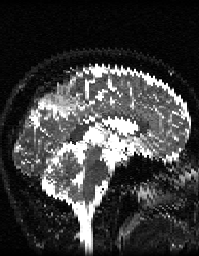
\includegraphics[width=.3\linewidth]{img/film_artifacts}&
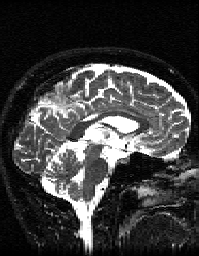
\includegraphics[width=.3\linewidth]{img/film_corrected}
\end{tabular}
\end{center}
\caption{Example of interleaved image before (left) and after (right)
  correction of motion artifacts using the {\tt film} tool. These are roughly
  mid-sagittal slices through a late-echo FSE image acquired in three
  interleaved passes.}
\label{fig:InterleavedExample}
\end{figure}

When MR images are acquired as multiple interleaved sparse image stacks
(``passes''), subject motion between the passes can lead to characteristic
artifacts in the final, interleaved image stack (see
Fig.~\ref{fig:InterleavedExample} for an example). CMTK implements an
algorithm for post-reconstruction correction of these
artifacts~\cite{RohlRadePfef:2008a} in the \verb|film| tool (for ``Fix
InterLeaved Motion'').

The \verb|film| tool operates in three stages: first, the interleaved image
stack is separated into the original passes, and all passes are co-registered
using rigid intensity-based registration to determine the inter-pass motion
parameters. Second, volume injection is used to obtain a coarse reconstructed,
motion-corrected image, which is then refined in the third stage using an
iterative inverse interpolation algorithm (see Ref.~\cite{RohlRadePfef:2008a}
for details).

For proper operation, the \verb|film| tool needs to be given the number of
passes in the interleaved images, for example for a three-pass image:
\begin{verbatim}
film --passes 3 input.nii corrected.nii
\end{verbatim}
In most cases, the through-plane acquisition direction can be guessed from the
data.

\subsection{MR Intensity Bias Field Correction}

CMTK implements a model-free algorithm for intensity bias field correction
based on minimization of image entropy~\cite{LikaVierPern:2001}. The
\verb|mrbias| tool, which implements this algorithm, is typically called as
follows:
\begin{verbatim}
mrbias --degree-mul 2 --mask foreground.nii spgr.nii spgr_corrected.nii
\end{verbatim}
which computes a second-order polynomial multiplicative bias
field. Computation is constrained via a (binary) mask that is read from the
\verb|foreground.nii| image. Alternatively, the tool can generate its own mask
via the \verb|--thresh-min| and  \verb|--thresh-max| command line parameters.

\begin{figure}[tbp]
\begin{center}
\begin{tabular}{cc}
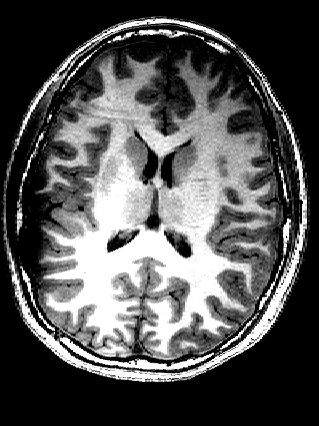
\includegraphics[width=.3\linewidth]{img/mrbias_orig}&
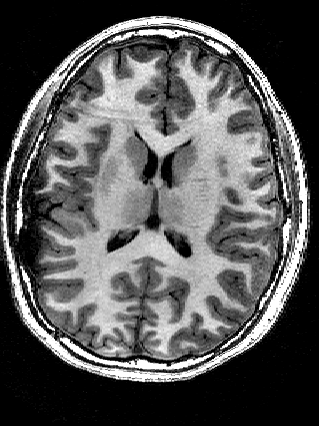
\includegraphics[width=.3\linewidth]{img/mrbias_corr}
\end{tabular}
\end{center}
\caption{Example of MR intensity bias field correction using a second-order
polynomial multiplicative bias field computed by the {\tt mrbias} tool and
applied to an SPGR image acquired at 3T.}
\label{fig:Mrbias}
\end{figure}

To generate foreground masks automatically, CMTK provides a very simple
``levelset-type'' segmentation tool:
\begin{verbatim}
levelset spgr.nii foreground.nii
\end{verbatim}
In very broad terms, the tool implements an extreme simplification of the
algorithm for segmentation without edges by Chan \& Vese~\cite{ChanVese:2001}.

\begin{figure}[tb]
\begin{center}
\begin{tabular}{ccc}
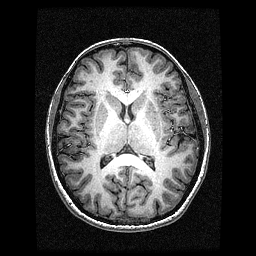
\includegraphics[width=.3\linewidth]{img/levelset_spgr_spgr}&
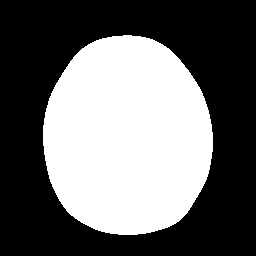
\includegraphics[width=.3\linewidth]{img/levelset_spgr_mask}&
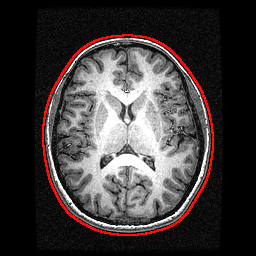
\includegraphics[width=.3\linewidth]{img/levelset_spgr_ovl} \\
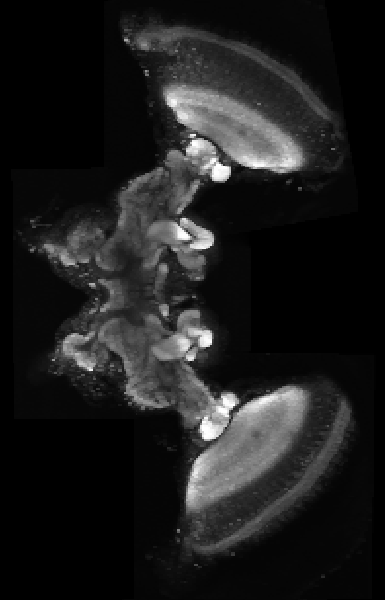
\includegraphics[width=.3\linewidth]{img/levelset_locust_clsm}&
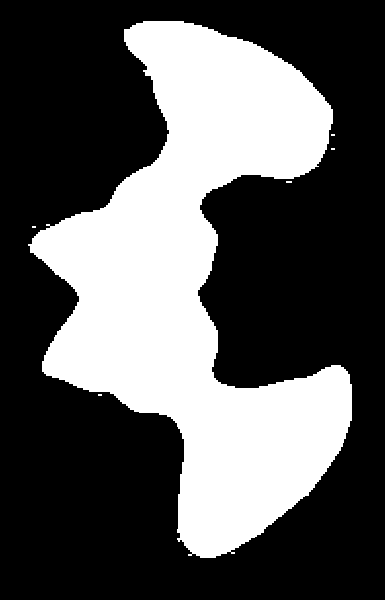
\includegraphics[width=.3\linewidth]{img/levelset_locust_mask}&
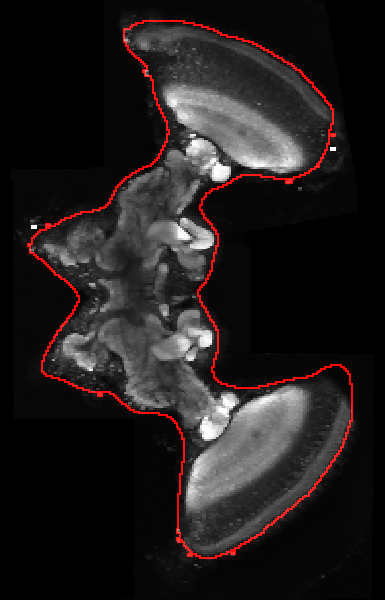
\includegraphics[width=.3\linewidth]{img/levelset_locust_ovl}
\end{tabular}
\end{center}
\caption{Examples of foreground/background segmentation using the {\tt
levelset} tool. {\em Top row:\/} SPGR image acquired at 3T. {\em Bottom
row:\/} fluorescent confocal laser scanning microscopy image of a locust
brain. Both examples were computed by running the {\tt levelset} tool with
default settings and no image-specific parameters.}
\label{fig:Levelset}
\end{figure}

\subsection{Affine Image Registration}

The basic pairwise image registration tool in CMTK, \verb|registration|,
implements an algorithm similar to the multi-resolution algorithm by Studholme
{\em et al.\/}~\cite{StudHillHawk:1997}. More technical detail about our
implementation in particular can be found in Ref.~\cite{Rohlfing:2000}, albeit
only in German.

In order to compute an affine registration between two images, the
registration tool can be run as follows:
\begin{verbatim}
registration --initxlate --dofs 6,9 --auto-multi-level 4 \
        -o affine.xform ref.nii flt.nii
\end{verbatim}
This performs a registration of the floating image, \verb|flt.nii|, to the
reference image, \verb|ref.nii|, where all optimization and image resampling
parameters are automatically determined for a 4-level multi-resolution
procedure. 

At each resolution level, the registration first optimizes 6 degrees of
freedom (DOF), i.e., translation and rotation of a 3D rigid
transformation. Afterwards, 9 DOFs are optimized, i.e., three anisotropic
scale factors in addition to the translational and rotational
parameters. Supported DOF numbers are: 0 (no registration, for testing),
3 (translation only), 6 (rigid: translation, rotation),  7 (similarity:
translation, rotation, global scale), 9 (translation, rotation, anisotropic
scale), and 12 (full affine: translation, rotation, scale, and shears).

By default, registration uses the normalized mutual
information~\cite{StudHillHawk:1999} image similarity measure. Other available
similarity measures are: standard mutual
information~\cite{MaesCollVand:1997,WellViolAtsu:1996} (\verb|--mi|), mean
squared difference (\verb|--msd|), normalized cross-correlation
(\verb|--ncc|), and correlation ratio~\cite{RochMalaPenn:1998a} (\verb|--cr|)

In the above example, the registration transformation is initialized (via
\verb|--initxlate|) by translating the floating image's center to that of the
reference image. For more complex initializations, the
\verb|make_initial_affine| tool can be used, which supports centers of mass,
principal axes~\cite{AlpeBradKenn:1990}, and image orientation vectors (e.g.,
as provided by the original DICOM data).

For example, in order to first initialize a transformation using principal
axes and then use the result as the initial transformation for intensity-based
refinement, one would use the following sequence of commands:
\begin{verbatim}
make_initial_xform --principal-axes ref.nii flt.nii initial.xform
registration --initial initial.xform --dofs 6,9 --auto-multi-level 4 \
        -o affine.xform ref.nii flt.nii
\end{verbatim}

\subsection{Nonrigid Image Registration}

Pairwise nonrigid image registration in CMTK implements an algorithm
introduced by Rueckert {\em et al.\/}~\cite{RuecSonoHaye:1999}, which uses
as its transformation model multi-resolution free-form deformations based on
cubic spline interpolation between sparse, uniformly distributed control
points. Our particular implementation, which uses SMP parallelism to take
advantage of multi-CPU systems, was described in Ref.~\cite{RohlMaur:2003}.

A very simple nonrigid registration using a 40\,mm control point grid,
registering floating image \verb|flt.nii| to reference image \verb|ref.nii|
based on an affine transformation \verb|affine.xform| can be run as follows:
\begin{verbatim}
warp -o ffd40.xform --grid-spacing 40 --initial affine.xform ref.nii flt.nii
\end{verbatim}
Typically, however, one would want to run a more sophisticated multi-level
deformation, say with three refinements (each reducing the grid spacing by
1/2 for a final spacing of 5\,mm), and constrain the deformation using grid
bending energy:
\begin{verbatim}
warp -o ffd5.xform --grid-spacing 40 --refine 3 --energy-weight 1e-1 \
        --initial affine.xform ref.nii flt.nii
\end{verbatim}
To prevent folding of the deformation grid, it is possible to instead
constrain the Jacobian determinant of the deformation to be nonzero, which is
achieved by changing the above command as follows:
\begin{verbatim}
warp -o ffd5.xform --grid-spacing 40 --refine 3 --jacobian-weight 1e-5 \
        --initial affine.xform ref.nii flt.nii
\end{verbatim}

\subsection{Reformating Registered Images}

To reformat the registered floating image following the examples in
the previous section, CMTK
\begin{verbatim}
reformatx  -o reformat.nii --floating flt.nii ref.nii ffd5.xform
\end{verbatim}
The somewhat unintiutive order of arguments on the command line is due to the
versatility of the \verb|reformatx| tool, which allows for the concatenation
of arbitrary transformations (and their inverses), such as
\begin{verbatim}
reformatx  -o reformat.nii --floating img3.nii \
        img1.nii img1_to_2.xform --inverse img3_to_2.xform
\end{verbatim} 
By default, \verb|reformatx| uses trilinear interpolation, but it also
supports cubic (\verb|--cubic|) and cosine-windowed sinc
(\verb|--sinc-cosine|) interpolation for intensity images, partial volume
interpolation~\cite{MaesCollVand:1997} (\verb|--pvi|) for label images, and
nearest neighbor (\verb|--nn|) interpolation for all types of images.

\subsection{Jacobian Determinant Maps}

\begin{verbatim}
reformatx  -o jacobian.nii time1.nii --jacobian time1_to_time2.xform
\end{verbatim}

\begin{verbatim}
reformatx  -o jacobian.nii atlas.nii \
        atlas_to_time1.xform --jacobian time1_to_time2.xform
\end{verbatim}

\subsection{Statistical Testing}

\subsection{General Linear Modeling}

\subsection{Atlas-based Segmentation}

\section{Atlas Construction}

\subsection{Iterative Shape Averaging}

\cite{RohlBranMaur:2001}
\cite{KuryRohlKrof:2008,BranRohlRyba:2005}

\subsection{Averaging Pairwise Correspondences}

\cite{GuimMeunThir:2000}

\subsection{Groupwise Population Registration}

\cite{Learned-Miller:2006}
\cite{BalcGollShen:2007}
\cite{RohlZahrSull:2008,RohlZahrSull:2010}

\section*{Acknowledgments}

Much of the effort required to get CMTK ready for release as open source
software was performed by Mike Hasak at SRI. Calvin R. Maurer, Jr., wrote the
original implementation of his linear-time algorithm for the Euclidean
distance transform~\cite{MaurQiRagh:2003}, which
\verb|cmtk::UniformDistanceMap| is based on, and kindly agreed to distribution
of this derived code under the GPL. Likewise, Daniel Russakoff kindly agreed
to GPL licensing of code he wrote for entropy computation based on covariance
matrices, as he used it in his work on Regional Mutual
Information~\cite{RussTomaRohl:2004}. Greg Jefferis provided numerous bug
reports and fixes, including much of the details required to get CMTK compiled
and working on the MacOS platform.

%%%%%%%%%%%%%%%%%%%%%%%%%%%%%%%%%%%%%%%%%
%
%  Insert the bibliography using BibTeX
%
%%%%%%%%%%%%%%%%%%%%%%%%%%%%%%%%%%%%%%%%%

\bibliographystyle{UserGuideCMTK}
\bibliography{cmtk}

\end{document}
